\section{Miscellaneous Items}

\vspace{5mm}

\subsection*{The Die of Ruh'Brex} 

\begin{center}
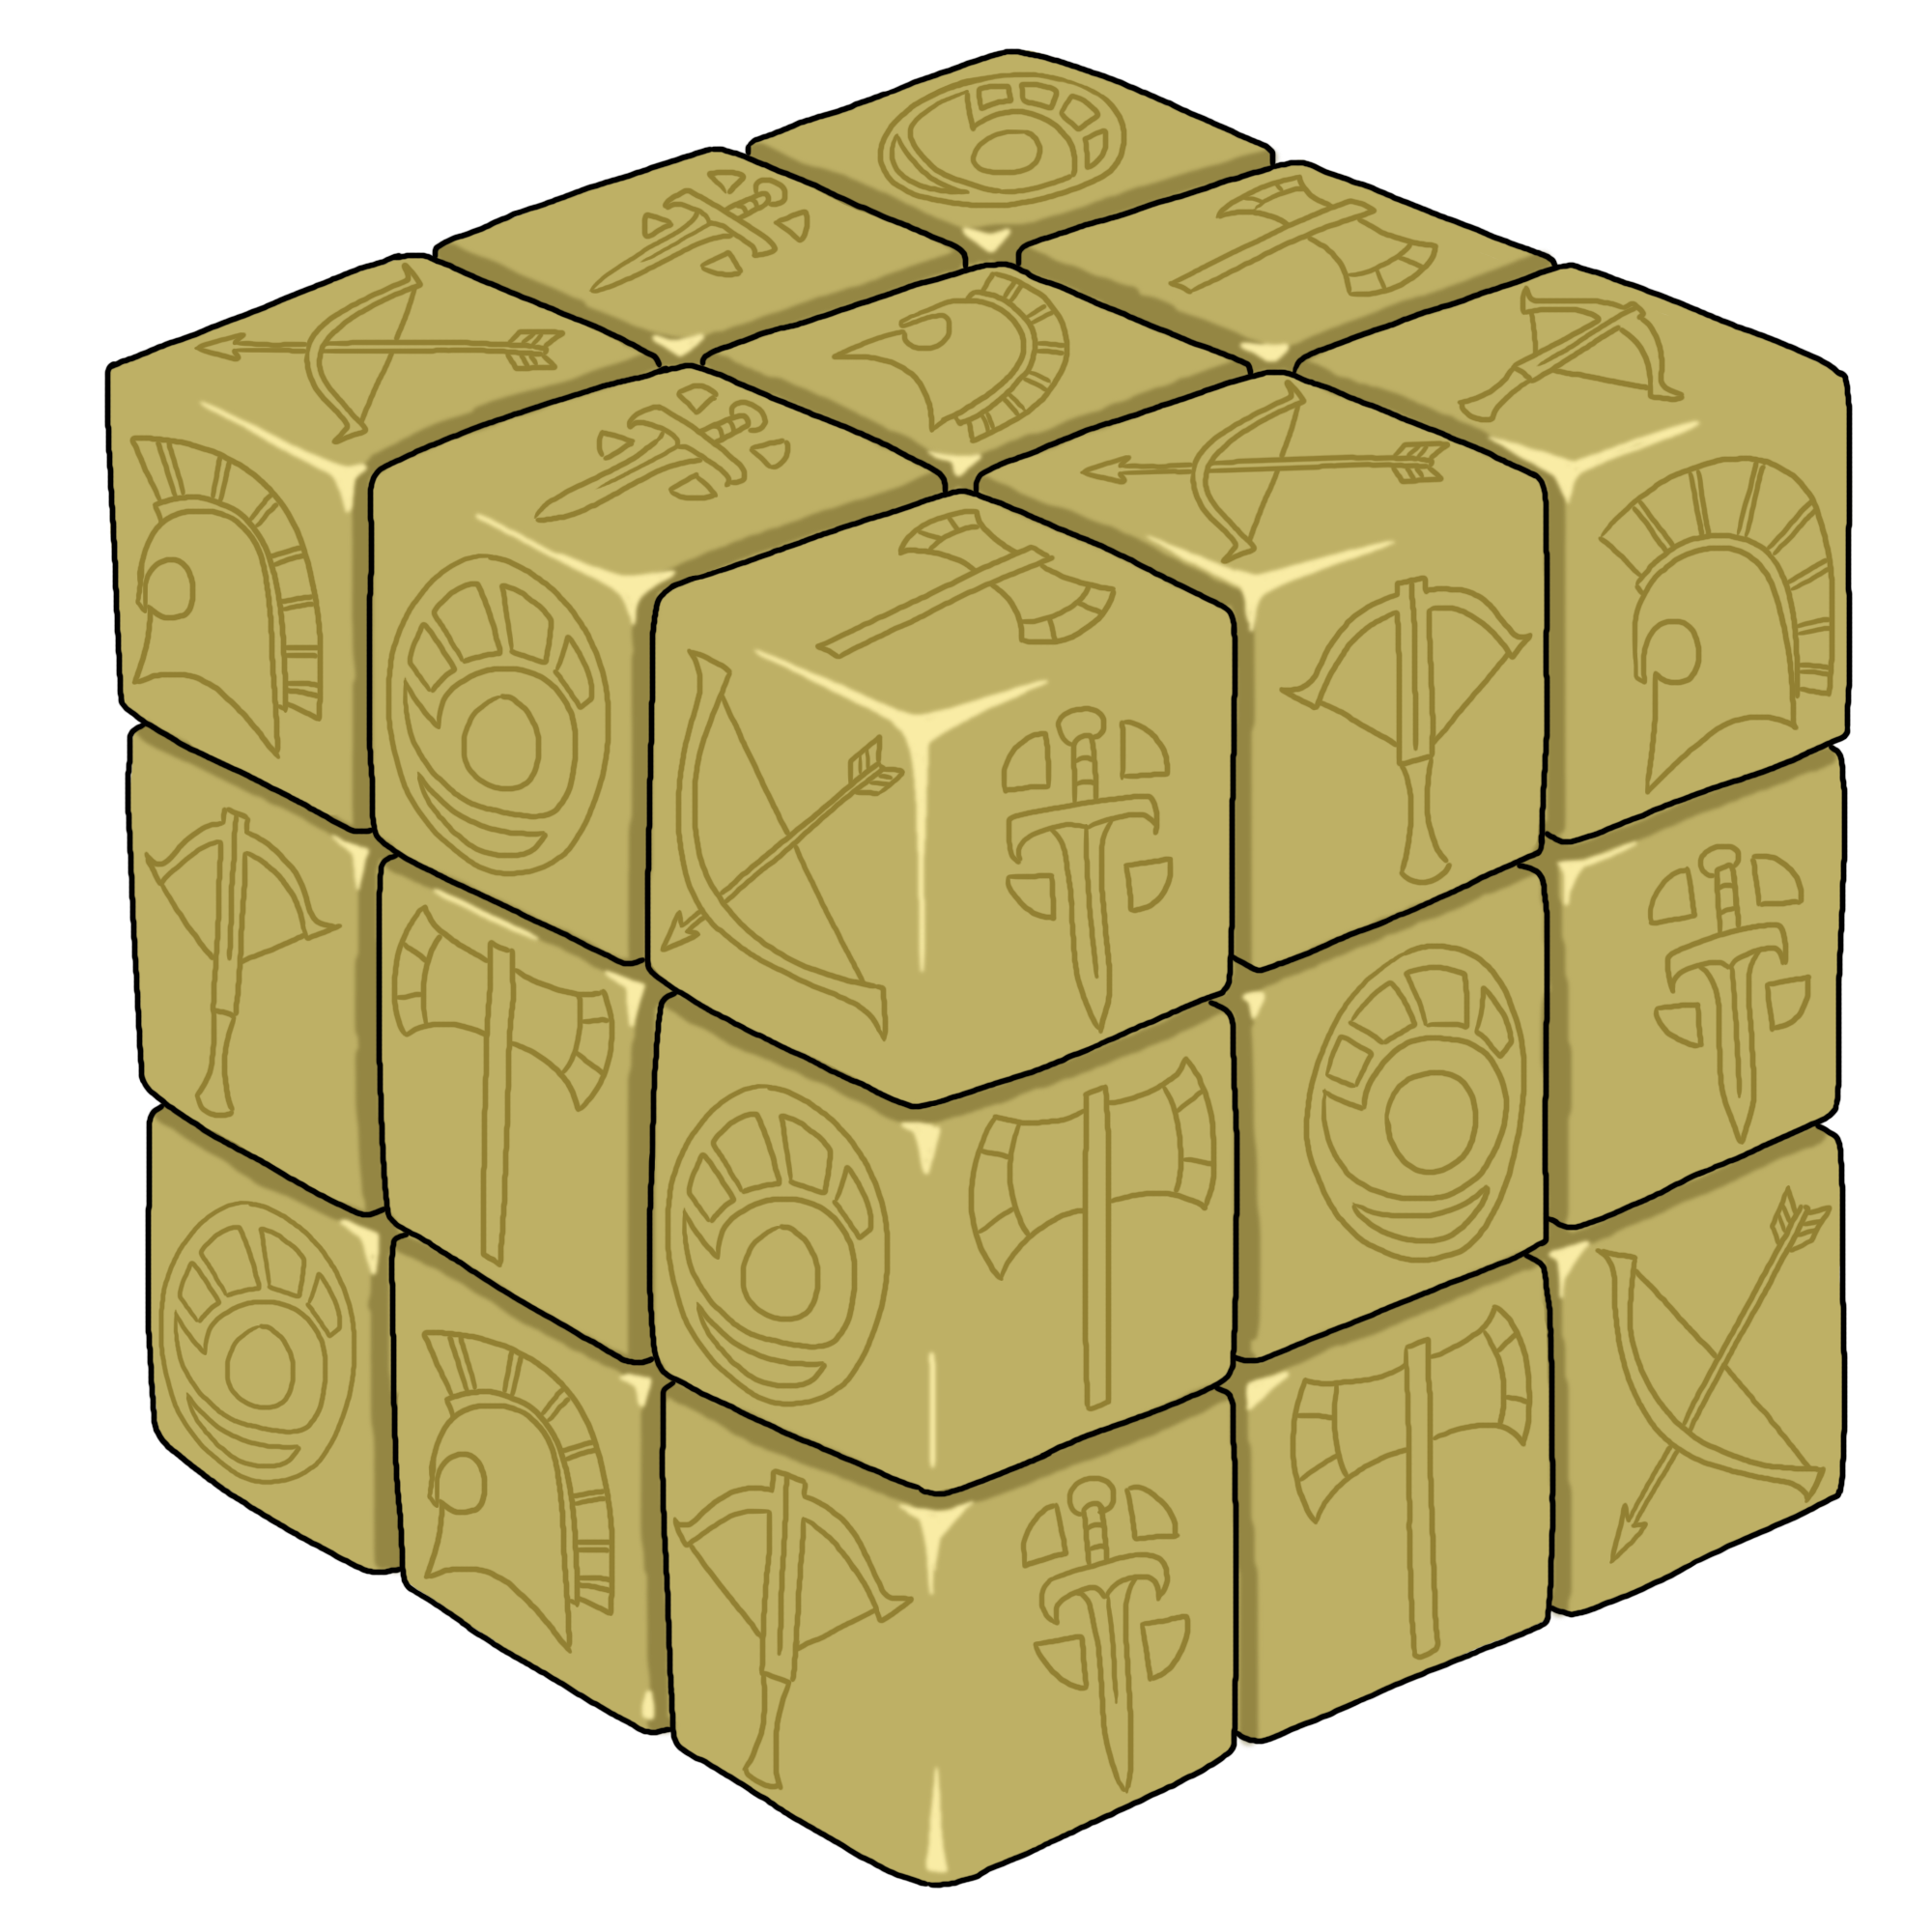
\includegraphics[width=80mm]{./content/img/dieRubriks.png}
\begin{figure}[h]
\end{figure}
\end{center}

\noindent 

Text

\begin{DndTable}[color=PhbLightCyan]{cX}
  \textbf{No.} & \textbf{Function} \\
  1           & Lockdown  \\
  2           & Locate Artefact \\
  6           & Invisibility \\
  7           & Summon TEST Goat \\
  8           & Fly \\
  11           & Motivator \\
  13           & Teleport \\
  14           & Rhu'Brex's Portable Domicile \\
  17           & Minor Time Stop \\
  18           & Increase Travel Speed \\
  19           & Healing \\
  H3           & Summon Monster\\
  H5           & Golbe of invulnerability\\
  H8           & Wish (10,000 year cooldown) \\
\end{DndTable}

\smallskip

\subsection*{Stone of Unthala} 

\begin{center}
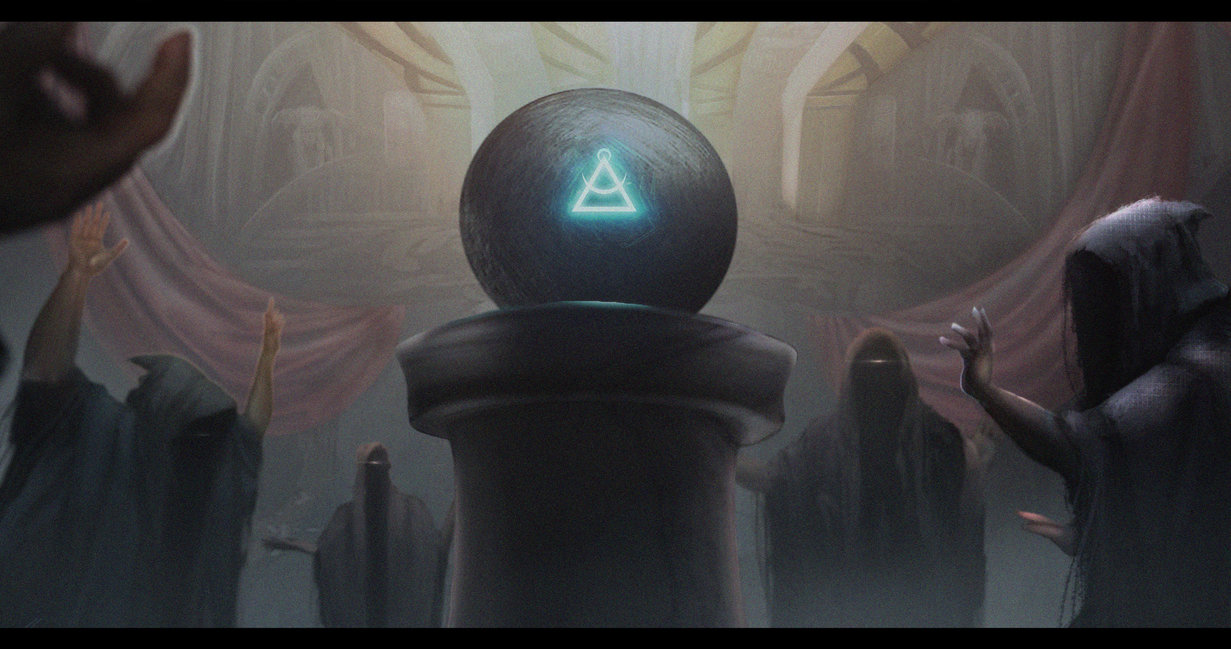
\includegraphics[width=80mm]{./content/img/unthala1.jpg}
\begin{figure}[h]
\end{figure}
\end{center}

\noindent 

A big stone, about the size of two fists. Allows communication with Laz, may enhance powers of those near it.

\smallskip

\subsection*{Ring of Deadly Visage} 

\noindent 

A ring 	Makes the wearer look corpsefied 	Flukely found in a Mine

\smallskip

\subsection*{Slab of Inthun} 

\noindent 

Big stone slab deep in the basement of the church in Logarsk 	Seems to either 1) Kill the user strapped to it or 2) Imbue them with awesome power, including nigh-on invulnerability - works better with kids 	We stumbled upon it, but it's further elaborated in On Power and Magick

\begin{DndComment}{Extract from ''On Power and Magick"}
In debates amongst scholars between the dangers and power of magic the slab of enchanted rock known as the Inthun is one of the most contentious. Its power is undeniably vast, imbuing a being with great strength, innate magical abilities and nigh-on invulnerability, however the risks are great. Most who bind themselves to the stone in search of power and rendered asunder by the power within. Few are willing to risk near certain death to achieve this power.

Some scholars assert that a younger body may be more adaptable to the flow of power; however what mother would sacrifice their child to such terrible danger? There are further concerns around the effects of the power on the mind. Those few who have come through the rite unscathed have a tendency to madness – few will forget the ravages of Gillius, a man so corrupted by power that the gods themselves had to intervene to stop him. Other scholars, of course, argue that only those who are unstable and unhinged dare to attempt to gain the power. There are too few cases for a stringent argument to be made either way, and the opportunity for true study is unlikely to arise.
\end{DndComment}

\smallskip

\subsection*{Assassin's Teapot} 

\begin{center}
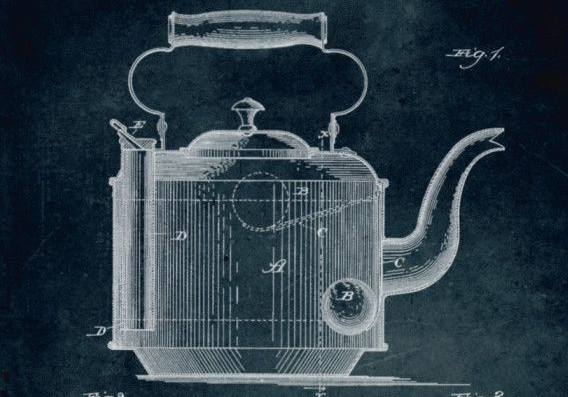
\includegraphics[width=80mm]{./content/img/teapot2.jpg}
\begin{figure}[h]
\end{figure}
\end{center}

\noindent 

A teapot with a normal chamber (for tea or similar) and a second, secret one, that contains poison. Uniquely, this teapot produces its own poison. 	The poison from this pot can be served, dealing hefty damage to the imbiber (5d10 - DC15 con save for half, fall unconcious for 1 hour on fail) or applied to a weapon (or 20 pieces of ammunition), where it deals 1d6 poison damage. The poison evaporates after an hour - whether in the teapot, a container or applied to a weapon.

\smallskip

\subsection*{The Burner} 

\begin{center}
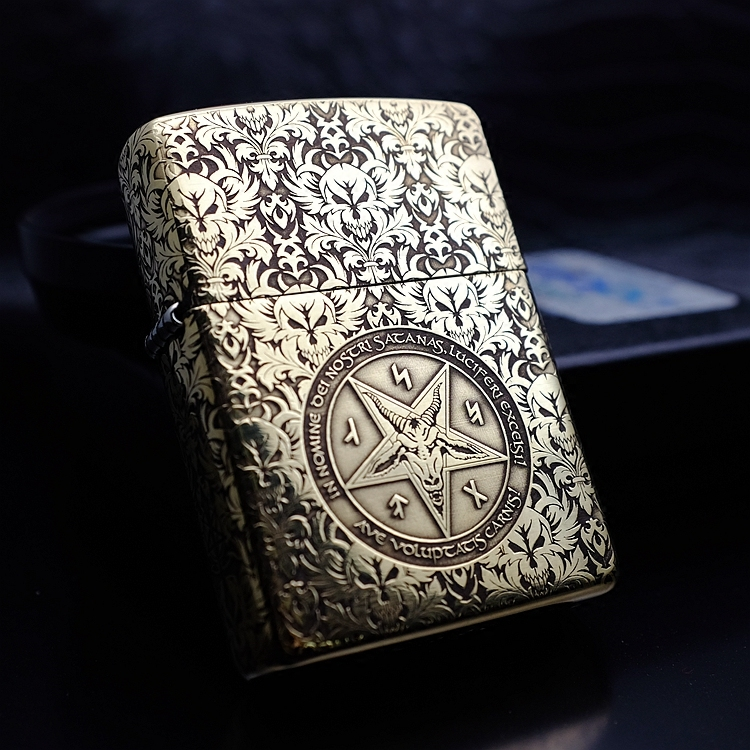
\includegraphics[width=80mm]{./content/img/lighter.jpeg}
\begin{figure}[h]
\end{figure}
\end{center}

\noindent 

The original book burners lighter, though it may in fact have been more a tool for study and exploration - has various powers around flame and bears an inscription in ancient velterran. 	

The lighter can produce a small ball of flame that emits light and can be hurled offensively (Produce Flame). Additionally, once per day if the flame is wafted under a weapon (elemental weapon(fire)) or some ammunition (flame arrows) it will imbue them with flame. Lastly, if the inscription is read, any writing that was written to intentionally mislead or obfuscate the truth will glow red if under the flame of this light.

\smallskip

\subsection*{Excalibrum (AKA Starmetal)} 

\begin{center}
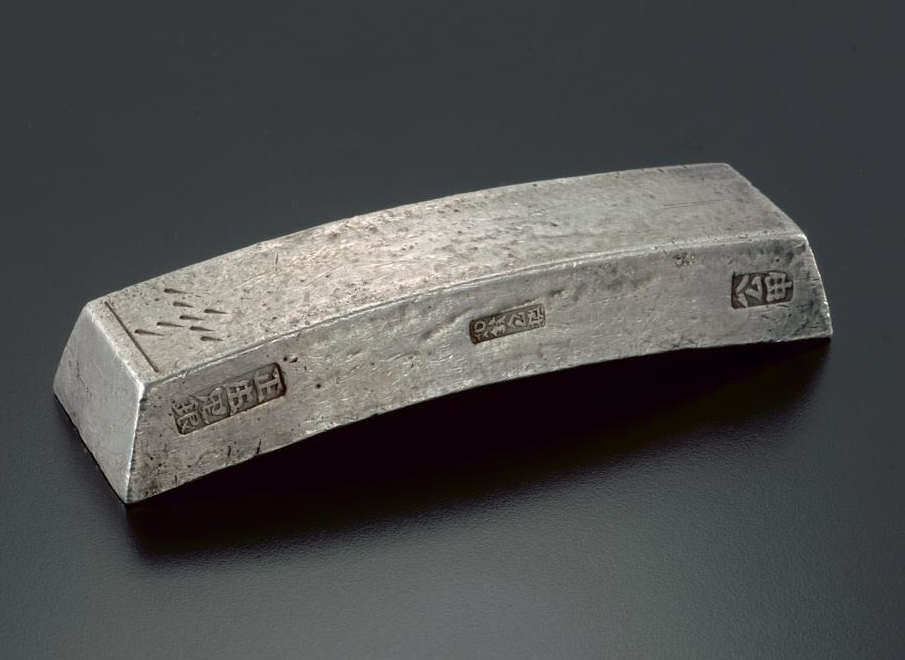
\includegraphics[width=80mm]{./content/img/excal3.jpg}
\begin{figure}[h]
\end{figure}
\end{center}

\noindent 

A gift from the gods, a special metal or alloy that can be found in falling stars - called Meteorites - seems capable of harming those blessed by the Inthun, so hopefully makes potent weapons. Needs a master smith

\begin{DndComment}{Extract from scraps of text}
The rarest of metals, the starmetal known as Exallibrum… only known source being from the meteorite that fell… only the most master forgers can work the metal….one of the few known things that can harm…this gift from the gods…indeed the Inthun itself…seek to grow rich from the rare metal they have founded themselves above…must take great care…but the rewards are magnificent.
\end{DndComment}

\smallskip


\clearpage